\section{Introduction}
The work presented in this thesis, being experimental in nature, hinges on numerous experimental techniques.
The fundamental components of this work rely on extensive use of X-ray diffraction (XRD) and transmission electron microscopy (TEM) in both standard and novel ways.
These techniques will be examined and explained in some detail, as their novel usage is integral to the work presented here.
Several other experimental techniques are also utilized in this work, but they are used in their everyday implementations as seen in the literature.
These experimental techniques will be discussed only briefly.
The two primary growth techniques used in this work will also be described, however as this work concentrates on epitaxy as a general phenomenon, the intricacies and parameter spaces of these techniques will not be considered again for brevity.

\section{X-Ray}
X-rays are high energy photons, generated from the transitions of electrons between their core shell energy levels and bremsstrahlung radiation (the deceleration of electrons).
X-rays have weak interactions with matter, being absorbed or perturbed only slightly upon passing through it.
X-rays have wavelengths comparable with the typical spacings between atoms in crystals, placing them as an ideal non-destructive probe for crystal structure.
In XRD, X-rays experience elastic scattering when interacting with the electrons surrounding atoms.
The scattering of X-rays, combined with the 3D periodic structure of atoms, results in constructive and destructive interference and X-ray diffraction\cite{zavalij}.
X-ray diffraction is fundamentally an interference phenomenon. 
For a set of planes within a crystal separated by some distance (d), they will diffract from those planes at an angle (\straighttheta) depending upon the wavelength (\textlambda{}), this is known as Bragg's law as in \cref{eqn:bragg}.
\begin{equation}
\label{eqn:bragg}
2d \sin(\theta) = n \lambda
\end{equation}
Bragg's law is identical to the phenomenon of thin film interference of visible light, only differing by the scale.
Bragg's law, while correct, is a one dimensional expression, in three dimensions it can be represented by the Laue equations as in \cref{eqn:lauea,eqn:laueb,eqn:lauec}.
The vectors \textbf{k\textsubscript{i}} and \textbf{k\textsubscript{0}} are the incident and outgoing X-ray beam, \((a,b,c)\) are the primitive vectors of the crystal lattice and \((h,k,l)\) are the reciprocal lattice indices.
Thus, for a given crystal with a fixed unit cell, there are only certain relationships between the incident and outgoing X-ray beams that satisfy the diffraction conditions, resulting in X-ray diffraction.
\begin{align}
 \mathbf{a} \cdot (\mathbf{k_0} - \mathbf{k_i}) = 2 \pi h \label{eqn:lauea} \\
 \mathbf{b} \cdot (\mathbf{k_0} - \mathbf{k_i}) = 2 \pi k \label{eqn:laueb} \\
 \mathbf{c} \cdot (\mathbf{k_0} - \mathbf{k_i}) = 2 \pi l \label{eqn:lauec}
\end{align}

A concept known as reciprocal, or momentum space, is a common construct used in solid state physics to discuss the properties of crystals and is intimately related to diffraction.
Reciprocal space can be visualized as a lattice of points, each representing a spacing present in the crystal, and the lattice having the same symmetry as the real crystal.
Reciprocal space is also the Fourier partner of the real space lattice of the crystal.
Reciprocal space provides an opportunity for an alternate expression of the conditions for diffraction, known as the Ewald construction.
The Ewald construction or Ewald sphere expresses the diffraction condition through the overlay of a sphere of radius 1/\textlambda{} pinned on its radius at the origin in reciprocal space, an incident X-ray beam (\textbf{k\textsubscript{i}}) entering the sphere.
The direction of the exiting diffraction beam is determined by the intersection of the surface of the sphere with the reciprocal lattice, as shown in \cref{fig:exp_xray_ewald}.
As a crystal is rotated (or the incoming beam is moved), the Ewald sphere will rotate about the reciprocal space origin, sweeping through reciprocal space and exciting diffraction conditions as the sphere coincides with lattice points.
The pinned rotation of the Ewald sphere about the origin means that only reciprocal lattice points with a radius from the origin of less than 2/\textlambda{} can be excited into diffraction, indicating the effective limitation of a given X-ray source, as well as why light is an ineffective diffraction probe.
\begin{figure}
 \centering 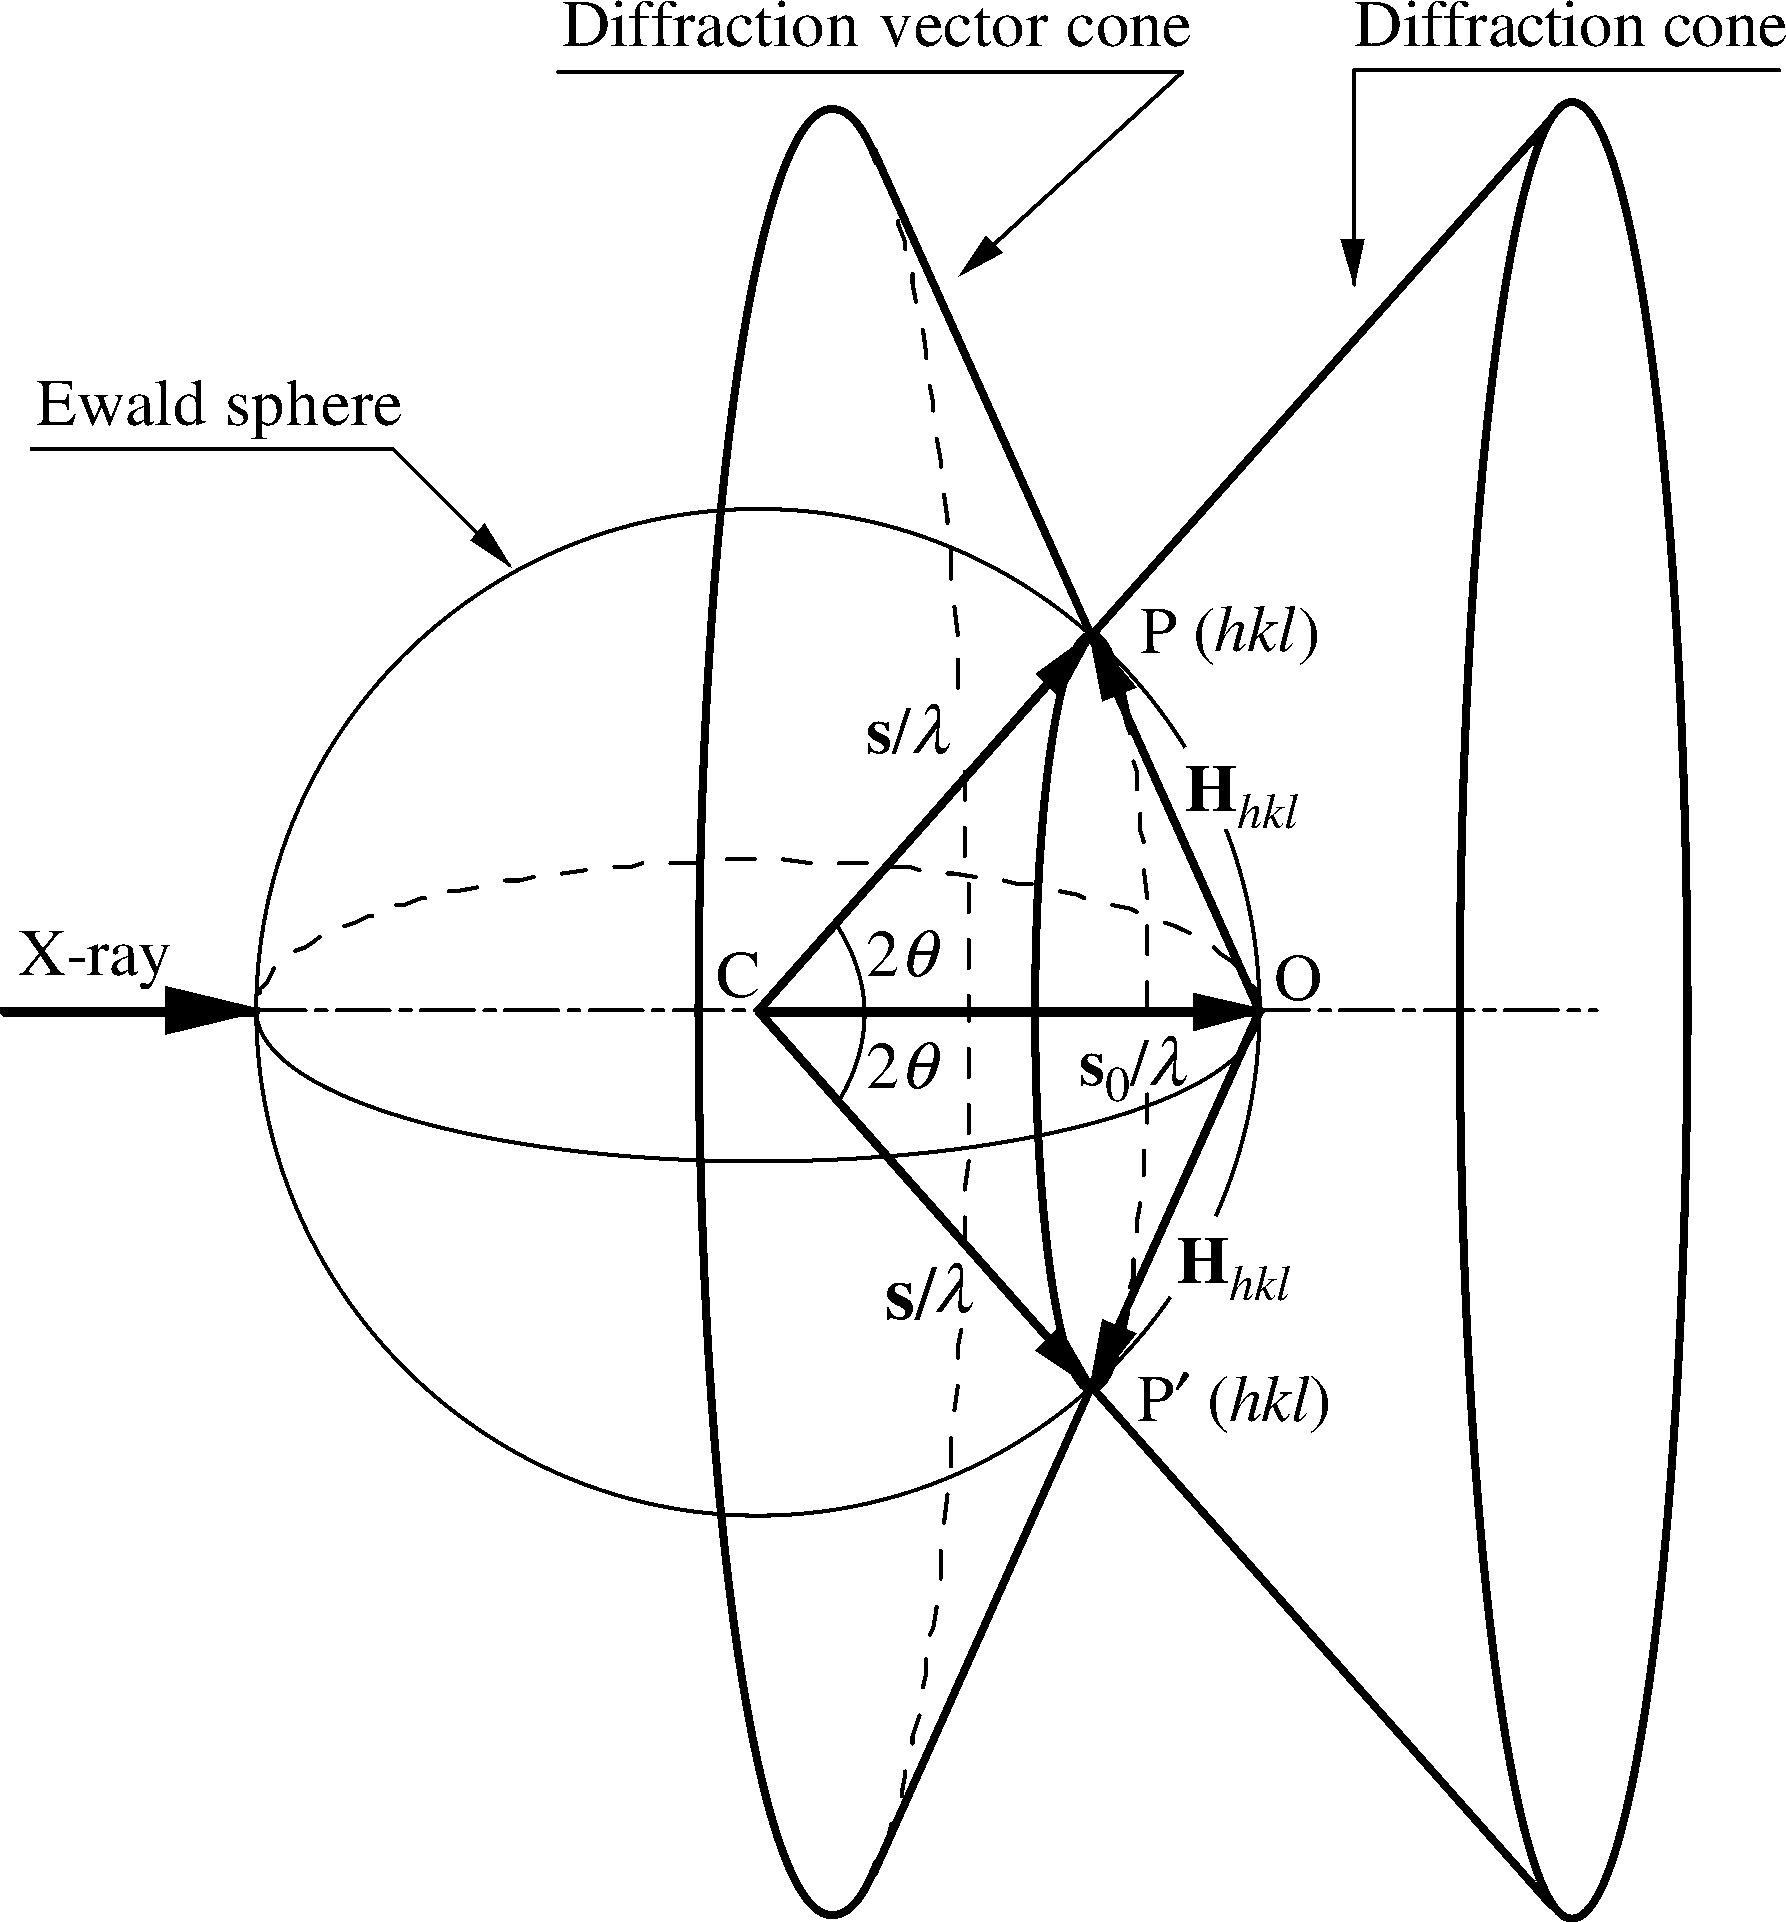
\includegraphics[width=0.6\textwidth]{exp_xray_ewald}
 \caption[Ewald sphere]{\label{fig:exp_xray_ewald}Ewald sphere construction of diffraction conditions (vector form of Laue equation) showing incoming X-ray beam to crystal (C) and the reflected and transmitted diffraction cones for a fixed (hkl) and 2\straighttheta{} (used with permission from \cite{He2009}).}
\end{figure}

\subsection{2DXRD --- Reciprocal Space Mapping}
\label{sec:2DXRD}
As shown by \cref{eqn:lauea,eqn:laueb,eqn:lauec} and \cref{fig:exp_xray_ewald}, there are a large number of orientations of a crystal which generate diffraction.
For the analysis of crystals, the lowest orders of crystal diffraction (small h,k,l) are the strongest, and provide the least ambiguous information, the they are also at the lowest 2\straighttheta{} values.
This still leaves a significant number of diffraction beams of interest to measure and provide structural information.
The na\"{\i}ve measurement technique for collecting this information involves taking a crystal and orienting an incoming X-ray beam, and a detector in configurations that satisfy \cref{eqn:lauea,eqn:laueb,eqn:lauec}.
Such measurements assume that the experimenter knows the orientation and unit cell of the crystal to a degree well enough to calculate those configurations.
If either of those pieces of information is unknown, the experimenter must instead sample the 4\textpi{} solid angle (usually only the upper 2\textpi{} half) of the angular space surrounding a crystal with enough resolution to intersect with the diffraction conditions of interest.
Such experiments, when performed using a typical X-ray point detector, take inordinate amounts of time, as the angular space is large and the point detector must count for a long time to achieve good counting statistics.

An alternate implementation of such a measurement process is with a 2D planar detector rather than a point detector.
A 2D X-ray detector can subtend a large section of the angular space surrounding a given experiment, potentially collecting information about a large section of reciprocal space with each frame it collects.
If the configuration is then swept through a range of diffraction conditions, the 2D detector will collect information about a wide swath of reciprocal space.
2DXRD techniques simultaneously collect information about the phase and symmetry of an unknown sample allowing that information to be then examined via a variety of techniques.

\subsubsection{Practical 2DXRD Measurement}
\begin{figure}
 \centering 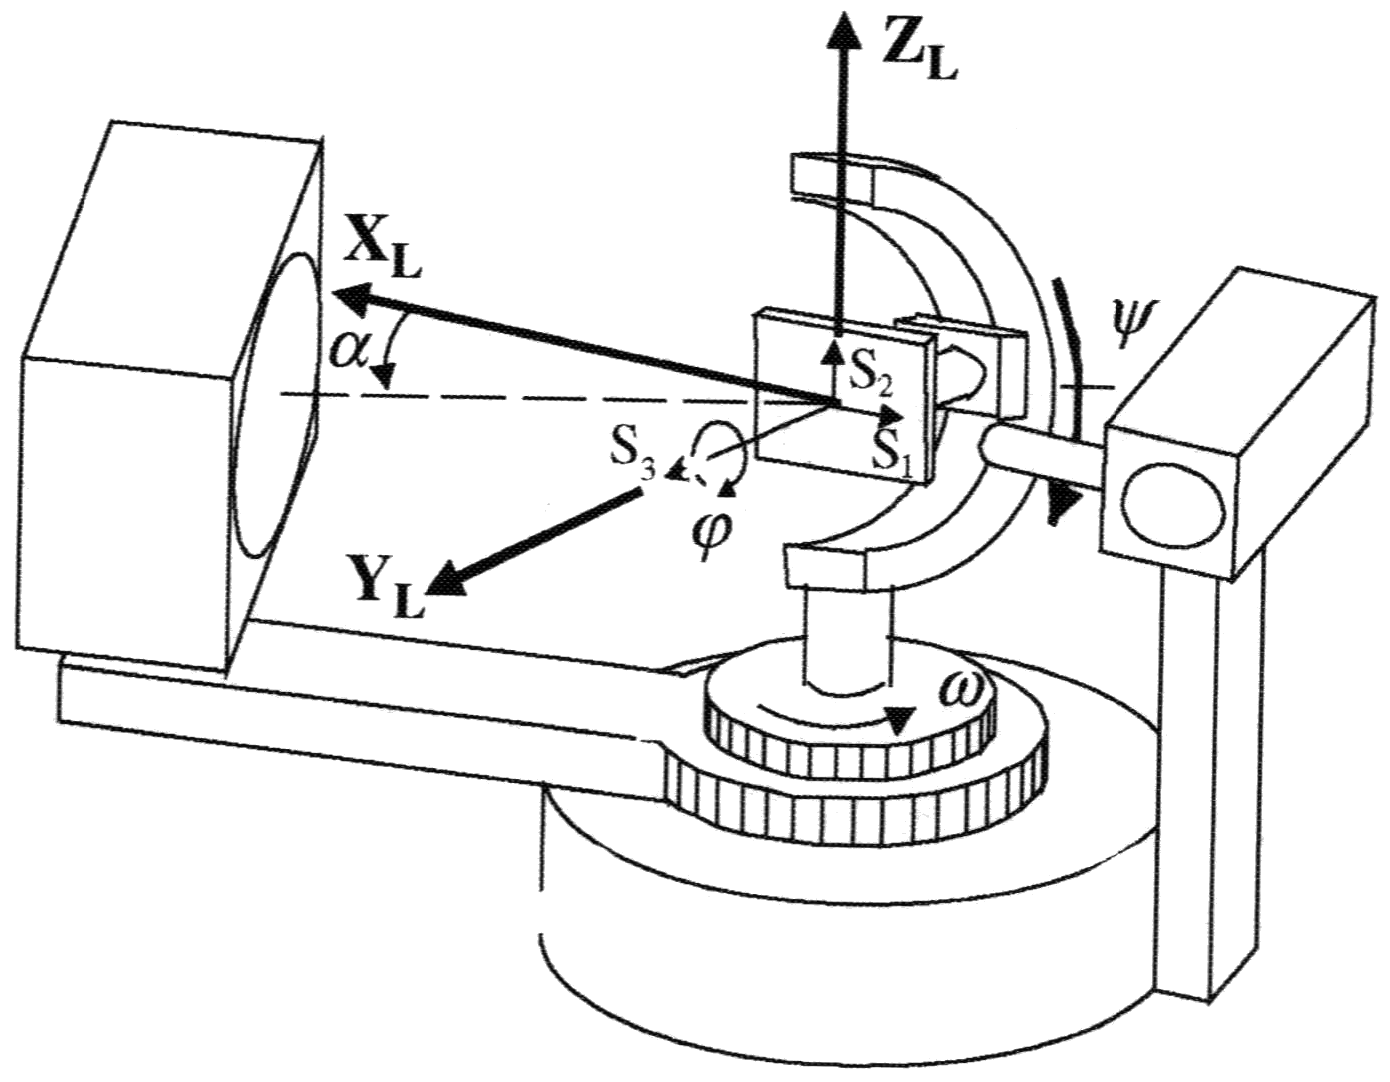
\includegraphics[width=0.8\textwidth]{exp_xray_machine}
 \caption[Typical 2DXRD experimental implementation]{\label{fig:exp_xray_machine}Standard configuration of a 2DXRD system with source, sample and detector, with the sample (S) and laboratory (L) coordinate systems labelled. Standard goiniometer angles are also labelled (used with permission from \cite{He2009}).}
\end{figure}
Practical 2DXRD measurements are achieved through the use of a multi-axis goiniometer, a device which maintains the sample at a central point while rotating its orientation relative to the X-ray source and detector.
For epitaxial crystals grown on crystalline substrates, a sample under measurement is placed in the goinometer with its surface normal oriented along the goiniometer's sample axis and a reference edge.
An X-ray source is placed on one arm of the goiniometer and the 2D detector is placed on the other arm.

A standard 2DXRD measurement is performed by configuring the goiniometer (\cref{fig:exp_xray_machine}) such that the X-ray source to 2D detector angle corresponds to a known or presumed low-order 2\straighttheta{} angle for the sample.
The sample is then rotated such that incident angle to the surface is shallow, typically less than 5\degree{}.
Such a beam configuration is ideal for collection of maximum diffraction information, however it can greatly increase the X-ray beam width (d\textsubscript{eff}), as shown in \cref{fig:exp_xray_beam_width} and \cref{eqn:exp_xray_beam_width}.
\begin{equation}
d_{eff} = \frac{d}{\sin{\alpha}} \label{eqn:exp_xray_beam_width}
\end{equation}
If the sample is of limited size, alternate measurement schemes must be computed.
The sample is then rotated about its surface normal while the 2D detector takes sequential images, a process known as a \textphi{}-scan.
By aligning the sample along 2\straighttheta{} in one dimension, and rotating the sample in a complimentary dimension, crystallographic reflections that contain the d-spacing corresponding to a range of 2\straighttheta{} around the selected value will be collected on the detector as they pass through their diffraction condition.
The number of frames exposed during this rotation determines the resolution along the \textchi direction in reciprocal space, while the pixel resolution of the 2DXRD detector, combined with of the 2DXRD detector distance determines the resolution in the 2\straighttheta{} dimension.
An additional scan of the sample while maintaining the 2\straighttheta{} configuration and scanning the X-ray beam incident angle is known as an \textomega{}-scan.
While the combination of these two scans collects only the reflections surrounding the centred 2\straighttheta{} of interest, if the measurement scheme successfully collects most of the reflections, the symmetry of the underlying system will allow any other reflections to be inferred, greatly reducing overall measurement time.
\begin{figure}
 \centering 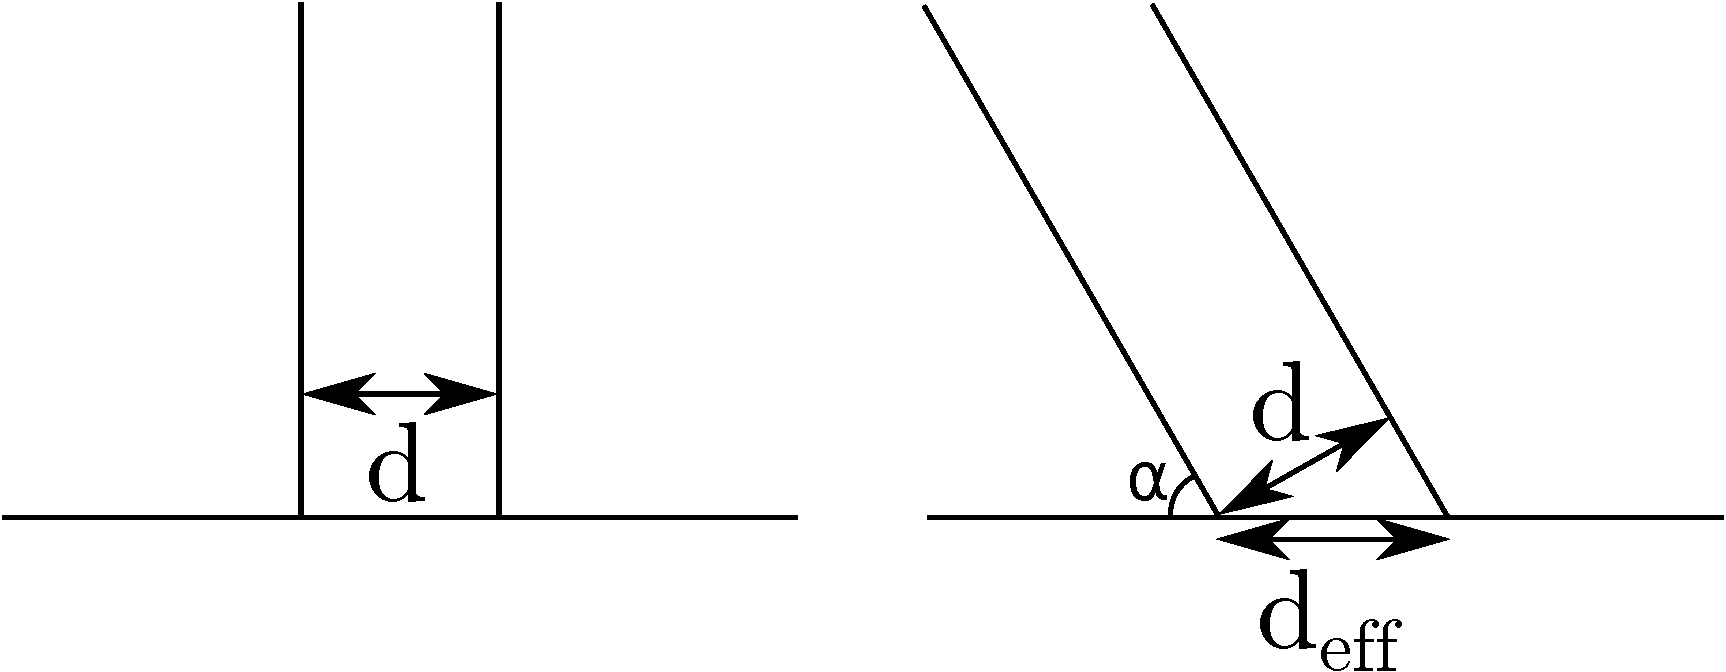
\includegraphics{exp_xrd_beam_width}
 \caption[X-Ray Beam Width]{\label{fig:exp_xray_beam_width}Comparison of beam width and effective beam width caused by inclination of sample.}
\end{figure}


As reciprocal space mapping is a process which operates in angular space, the distance to the detector is an important optimization parameter for 2DXRD measurements.
The distance the 2DXRD detector is situated away from sample will change the solid angle subtended by the detector.
Close detector distances allow the collection of more reciprocal space data in a given scan, at the expense of reducing the resolution due to finite pixel size, as well as increasing the risk of overlap for features close in 2\straighttheta{}.
For epitaxial thin films grown on lattice mismatched substrates, close detector distances can result in substrate and epitaxial crystal peaks overlapping, making interpretation difficult.

The last optimization parameter for 2DXRD scans is the time duration collecting each frame.
For a given brightness of X-ray source and thickness of material, the frame exposure times are ideally set to capture counts just below the maximum the electronics can achieve.
Maximizing the counts for the X-ray detector ensures optimum signal to noise for a given measurement.

\subsubsection{Interpretation of 2DXRD Measurements} Once a 2DXRD measurement has been taken, the resulting data consists of a series of 2D detector frames.
The exact number of frames is determined by the sampling resolution set during the 2DXRD scans.
Each frame is a snapshot of the diffraction intensity collected from the sample for the exact angular configuration in space stored with the frame.
A single 2DXRD frame (\cref{fig:exp_xray_frame}) which contains an X-ray diffraction peak can be analyzed via a number of integration techniques.
The two perpendicular pixel directions on the 2DXRD frames are transformed into two angular dimensions in the coordinate system of the sample, 2\straighttheta{} and \textchi{} \cite{He2009}.
The resulting frame is sliced into hyperbola with the x-direction of the frame corresponding to the radius (2\straighttheta{}) and a new dimension (\textchi{}) corresponding to the azimuthal direction along a given hyperbola.
\begin{figure}
 \centering 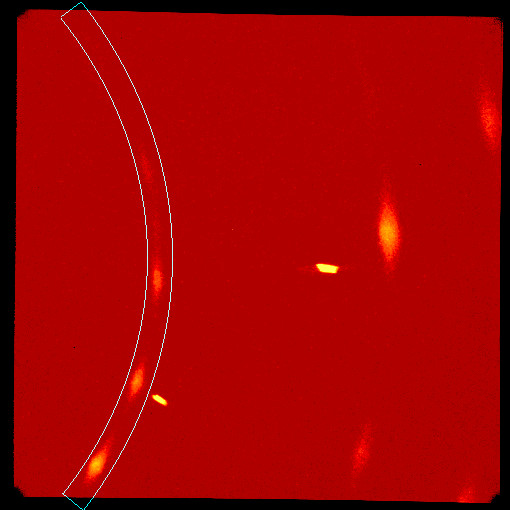
\includegraphics{exp_xray_frame}
 \caption[Example 2DXRD frame]{\label{fig:exp_xray_frame}An example X-ray frame with a conic section of fixed 2\straighttheta{} highlighted, also showing diffraction space coordinate directions \straighttheta{} and \textchi{}.}
\end{figure}

The data on a frame can be integrated in one dimensional plots along either dimension of the hyperbola.
Integration of the data along \textchi{} and plotting with respect to 2\straighttheta{} results in a pseudo-powder pattern similar to those taken in a common Bragg-Brantano XRD system, except it can be performed for diffraction peaks other than perpendicular to the substrate.
Such plots show the presence of d-spacings within the frame of interest, and their width.
Integration of data over a 2\straighttheta{} range and producing a one dimensional plot will show the spatial intensity distribution of a given diffraction peak.
An example 2DXRD frame, with labels of the two diffraction dimensions is shown in \cref{fig:exp_xray_frame}.

\subsubsection{Pole Figure Generation} While integration of the diffraction data on a single frame provides useful quantitative measures of the distribution of a diffraction peak in space, when many frames are collected the generation and interpretation of many frames is tedious and difficult to interpret.
Pole figure generation from a set of frames is a method of graphically representing the spatial extent of the diffraction intensity of a given d-spacing around a given sample.
Pole figures readily allow the interpretation of diffraction data to assess crystalinity, presence of phases and orientation relationships between a substrate and epitaxial crystal.
%\begin{figure}
%    \centering
%    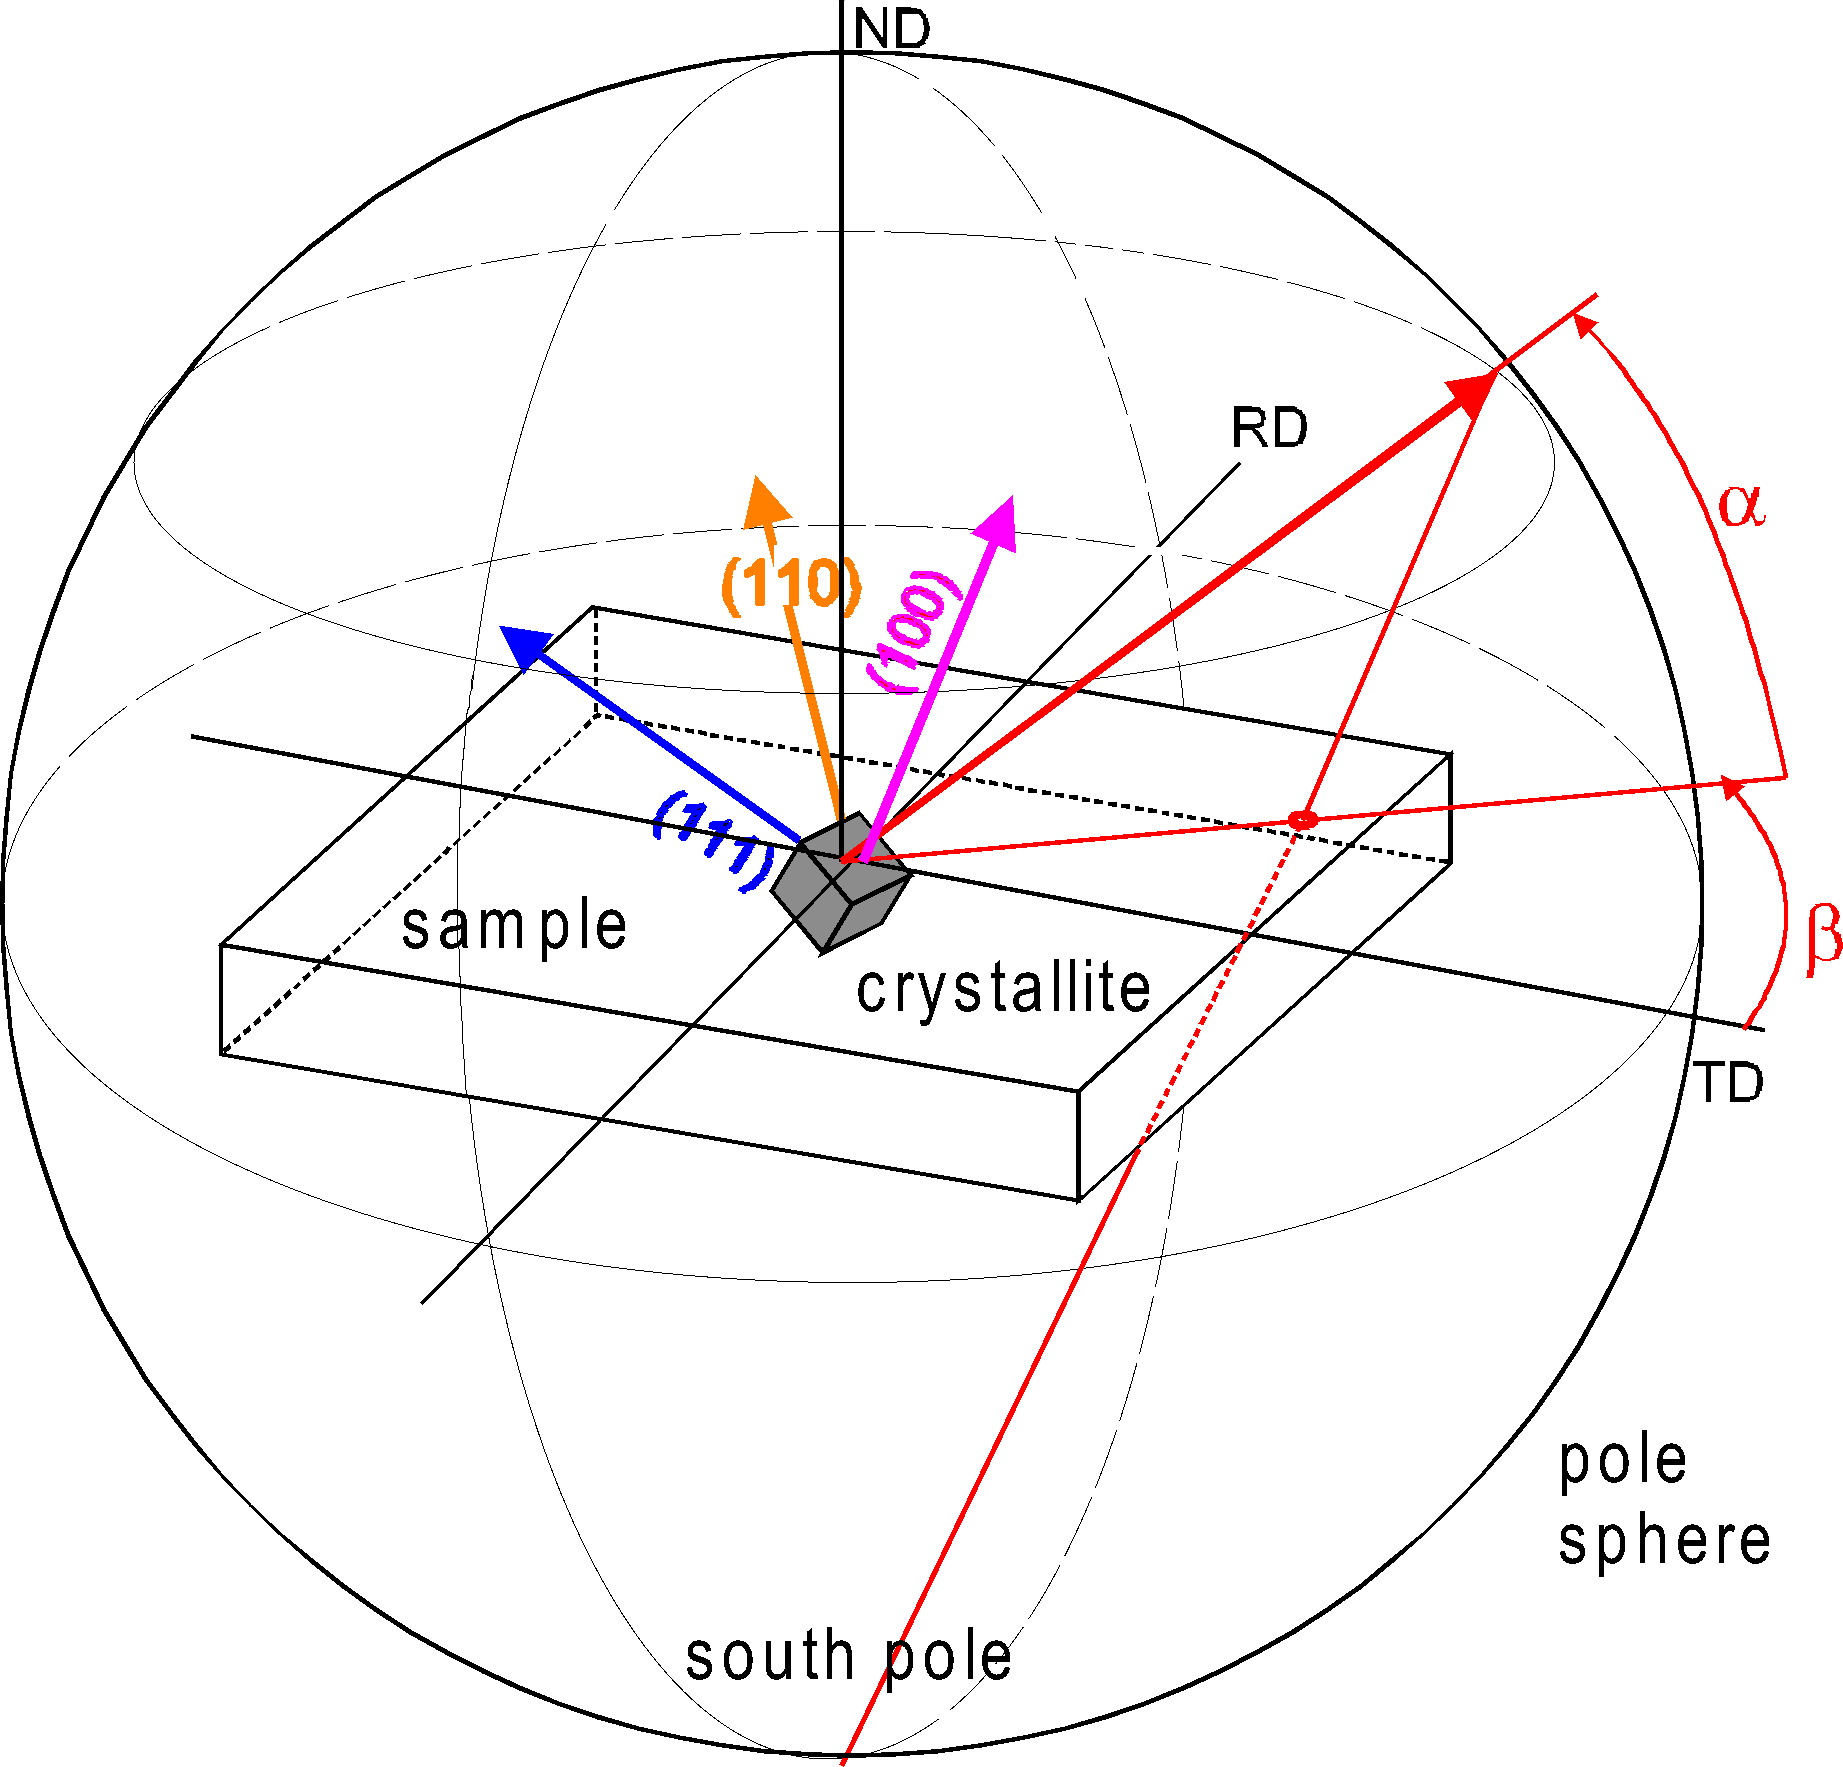
\includegraphics[width=0.7\textwidth]{exp_xray_polesphere}
%    \caption[Mapping of a unit cell to pole sphere]{\label{fig:exp_xray_polesphere}The pole sphere showing the origin of peaks in a pole figure and their relationship to the sample and an individual unit cell\cite{gadds_manual}}
%\end{figure}

To generate a pole figure from a collection of frames a 2\straighttheta{} and \textchi{} range are selected on the first frame of a series of frames.
Generally, such a range will include the maximum width of a single d-spacing of interest (such as \{111\}) and the entire extent of \textchi{} on the frame.
The range is integrated across 2\straighttheta{}, producing a one dimensional intensity scan.
The intensity scan from each frame is then mapped onto the pole sphere (\cref{fig:exp_xray_polefigure}) according to the frame orientation information, forming a geodesic line of intensity.
The pole sphere is a construction centred on the sample which maps the direction in space that diffraction intensity is collected by the detector.
As each frame is integrated, the surface of the pole sphere is painted with colour mapped intensity data.
The resulting sphere of data is then stereographically (angle preserving) projected onto a circle, resulting in a pole figure\cite{He2009}.
The pole figure is a polar diffraction intensity colour map with the radial direction represented by \textalpha{}, the angle from the top of the sphere and the azimutual direction \textphi{} is the in-plane orientation relative to the sample's \textphi{} zero orientation set during sample mounting.
An example pole figure mapping a single data point from the pole sphere is shown in \cref{fig:exp_xray_polefigure}.
\begin{figure}
 \centering 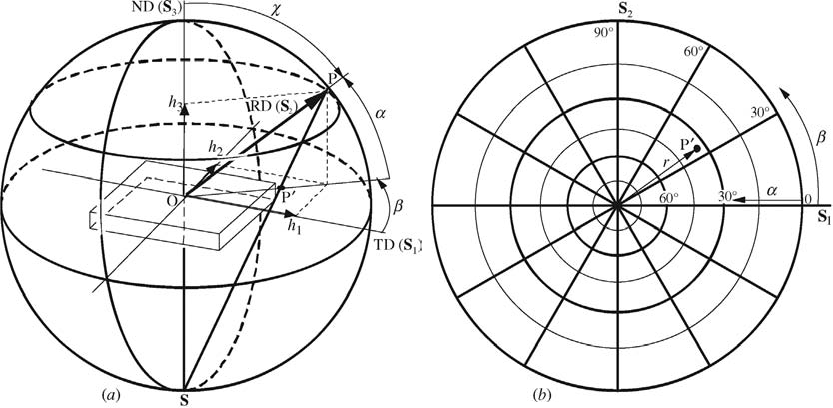
\includegraphics[width=\textwidth]{exp_xray_polefigure}
 \caption[Mapping of pole sphere to pole figure]{\label{fig:exp_xray_polefigure}Example mapping of pole sphere data points to pole figure (used with permission from \cite{He2009}).}
\end{figure}

\subsubsection{Interpretation and Simulation of Pole Figures} Once a pole figure has been generated the resulting graphical representation of the diffraction data must be interpreted in the context of the sample composition.
Generally, a pole figure will be generated for a low-index reflection (100,110,111) for both the epitaxial crystal and the substrate.
By generating two figures, the orientation relationship between the diffraction intensity produced by the grown crystal and the single crystal substrate can be examined by comparing the two figures.
\begin{figure}
 \centering \centering
 \begin{subfigure}[t]{0.53\textwidth}
  \centering 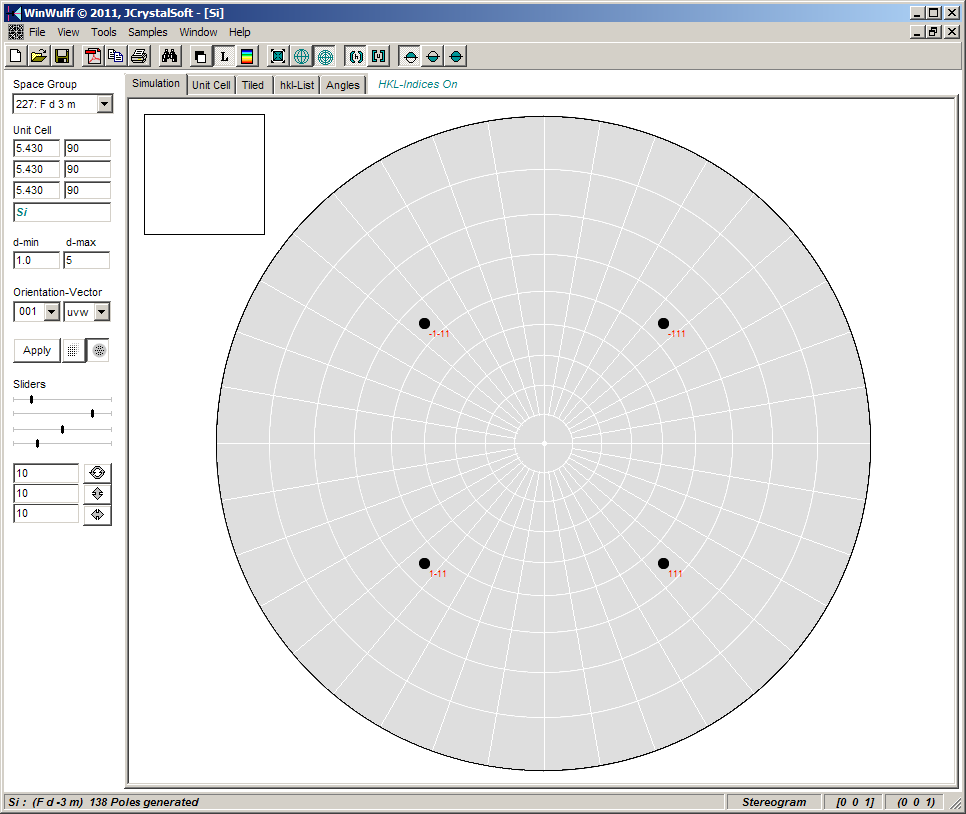
\includegraphics[width=\textwidth]{exp_xrd_winwulff_si_100}
  \caption{\label{fig:exp_xrd_winwulff_si_100}WinWulff (111) pole figure of (100)-up silicon.}
 \end{subfigure}\quad%
 \begin{subfigure}[t]{0.43\textwidth}
  \centering 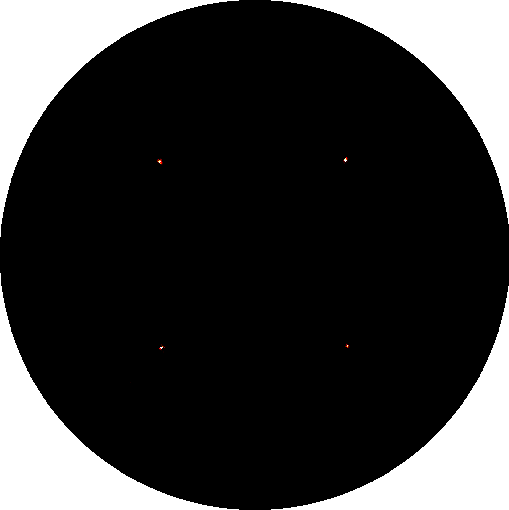
\includegraphics[width=\textwidth]{exp_xrd_si_100}
  \caption{\label{fig:exp_xrd_si_100}Experimentally generated (111) pole figure of (100)-up silicon.}
 \end{subfigure}
 \caption{\label{fig:exp_xray_winwulff}Comparison of WinWulff simulation and experimental single crystal silicon pole figure.}
\end{figure}

The first step for pole figure analysis is to examine the pole figure generated from the substrate low index reflection.
Since the substrate should be a single crystal, it is trivial to interpret it for its orientation information.
A single crystal pole figure of the substrate can be simulated by considering the space group (cubic, hexagonal, etc.), unit cell, and physical orientation (100-up, 111-up), calculating the surface normals of the d-spacing of interest, collecting them on a pole sphere and mapping them onto a pole figure.
This is conceptually identical to the generation of a pole figure from raw data, except the data is computed from a perfect crystal unit cell.
Such pole figures are simulated using a piece of software such as WinWulff\cite{Weber2006} as seen in \cref{fig:exp_xray_winwulff}, allowing interaction with the pole figure.
The pole figure generated from the data is then compared to the simulated pole figure and the simulation is manipulated by changing the orientation of the crystal until the two figures coincide.
The orientation information provided by the simulation software is now the same as the orientation of the measured crystal.
Such comparison provides the absolute orientation of the crystal in the diffractometer, and all other pole figures generated form the dataset can be referenced to that crystal.

Now that the substrate orientation is known, the pole figure generated from the data can be absolutely referenced to the substrate orientation.
If the epitaxial crystal is also a single crystal, the same trivial comparison process can be performed.
The resulting orientation of the eptitaxial crystal can be compared to the substrate, providing the epitaxial relationship.

For the case of systems which have non-ideal epitaxial growth, the pole figures likely contain diffraction intensity information from a number of crystalline sources.
This pole figure is the convolution of the pole figures for each of the components of the epitaxial crystal.
There are several features which arise in such pole figures which are characteristic of certain growth relationships.
A pole figure that, when generated, is uniform in intensity, or has intensity present everywhere with a broad distribution is characteristic of a strongly polycrystalline growth random in orientation, with no epitaxial relationship to the substrate, a simulated pole figure of such a situation is shown in \cref{fig:exp_xray_polefigure_examples}a.
Pole figures which contain bands of diffraction intensity which are rotationally symmetric about their centre are characteristic of a crystal that has a preferred stacking order in the vertical direction, but has no in-plane orientation, such an example is shown in \cref{fig:exp_xray_polefigure_examples}b.
Such preferred stacking orders, usually (111)-up, are a common occurrence when growing binary cubic materials.

The most difficult situation that occurs is when the generated pole figure contains multiple single crystal-like peaks.
The presence of single crystal-like peaks indicates a number of different orientations of the epitaxial crystal.
These epitaxial crystals are referred to as textured materials, an example of which is shown in \cref{fig:exp_xray_polefigure_examples}c.
For textured epitaxial crystals, there are number of possibilities for the cause of texturing during growth.
Faced centered cubic binary semiconductors have a propensity to have stacking faults or twins during growth.
The twinned crystallite will create new diffraction peaks in the pole figure, they will have a twin relationship with the host crystal about the twin direction (usually \{111\}).
Other textured epitaxial crystals may arise through multiple preferred growth relationships with the underlying substrate.
Such systems typically have pole figures where the symmetry of the overall pole figure reflects the substrate surface symmetry.
The example in \cref{fig:exp_xray_polefigure_examples}c is one of a (111)-up crystal (3-fold symmetry) on a (100) substrate (4-fold symmetry), showing \(3\times 4=12\) peaks.
\begin{figure}
 \centering 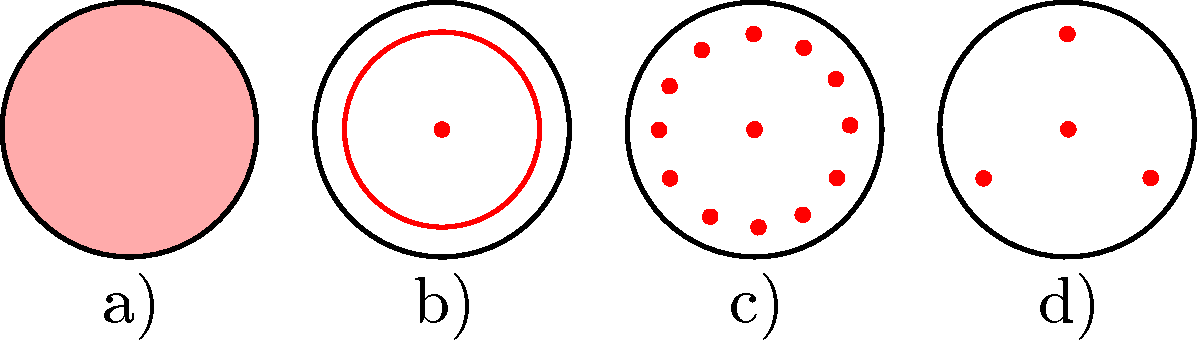
\includegraphics[width=\textwidth]{exp_xray_polefigure_examples}
 \caption[Example simulated pole figures]{\label{fig:exp_xray_polefigure_examples}Example (111) pole figures of a) Polycrystalline randomly oriented b) (111)-up in-plane random orientation c) (111)-up textured epitaxial d) (111)-up single crystal FCC cubic crystal.}
\end{figure}

Beyond the analysis of the symmetry of diffraction intensity, which identifies the crystallites present within a sample, the peak intensities within the pole figure provide a wealth of information about the epitaxial crystal.
Similar to the integration techniques applicable to raw 2DXRD frames, the diffraction intensity in a pole figure can be sliced and integrated in a number of ways.
The pole figure can be inspected by integrating the intensity in a given area, allowing comparison of individual diffraction peaks.
Pole figure intensity can also be integrated radially and plotted versus \textphi{}, providing information on the in-plane rotational misalignment of the selected epitaxial crystallites.
Finally, pole figure intensity can be integrated versus \textphi{} and plotted radially.

Plots of peak broadening from pole figures are particularly informative.
Broadening of diffraction peaks preferentially in the radial dimensions is a sign of strain present in a crystallite.
The radial location of a peak in a pole figure is determined by angular relationships of the unit cells of the sample, fixed angles are expected for a given crystal group (e.g.\ cubic).
Radial broadening in a pole figure is an indication that the unit cell has been distorted from its preferred shape.
Similarly, broadening in azimuthal directions indicates the individual crystallites sampled by the 2DXRD measurement have in-plane misalignment, similar to a textured film, but of much smaller extent.

\subsection{High Resolution XRD} While mapping reciprocal space provides much information about the phases and symmetries present in a given sample, the resolution available on such 2D detectors is limited in both the number of pixels, and the spacing between them.
In addition, the X-ray beam geometry associated with 2DXRD measurements introduces instrumental broadening into the measurements preventing careful inspection of small scale diffraction details.
To examine the small scale details of diffraction intensity, a different configuration must be implemented for the X-ray source and detector, this configuration is known as high resolution X-ray diffraction (HRXRD).
If the general landscape of reciprocal space (diffraction intensity) is known through the application of 2DXRD techniques, HRXRD can carefully sample small sections of reciprocal space with very high resolution.

Recall that for a perfect crystal, there is only a single configuration for which the diffraction condition will be satisfied, resulting in a highly intense diffraction peak with minimal spacial extent.
For a real sample, intensity distribution of individual diffraction peaks in reciprocal space provides information about the deviance from the ideal crystal.

Using HRXRD measurements, the precise d-spacing of a given material can be determined, showing whether a sample has its lowest energy structure or it is strained.
If the orientation of the sample can be controlled carefully, the d-spacing can be measured absolutely, otherwise, it can be measured relative to a known standard such as a single crystal substrate.
The broadening (spatial extent) of a HRXRD peak provides different information depending upon the dimension along which it is examined.
In the 2\straighttheta{} direction, the radial direction in reciprocal space, broadening indicates that the spacing of interest is a distribution of spacings within the region of the sample illuminated by X-rays.
Such distributions can indicate strain or compositional variation in the region of interest.
The broadness of the X-ray peak when a sample is rocked in the \textomega{} direction, while keeping 2\straighttheta{} fixed indicates that a given d-spacing has a distribution of orientations within the sample, usually indicating multiple crystallites.

\subsubsection{Practical HRXRD Measurement} To ensure the validity of HRXRD measurements of precise d-spacings and X-ray diffraction peak widths, the HRXRD system and its operation must satisfy several conditions.
These properties specifically deal with the properties of the X-ray source used in HRXRD, and the operation of the goiniometer in the rotation of the sample, source, and detector.

For practical HRXRD, the X-ray source must be monochromated far more than for general X-ray work.
Typical X-ray sources will contain bright peaks from multiple core electron levels, along with bremsstrahlung radiation, and will be monochromated with a single monochromator.
Such a source will still have an appreciable broadening in its peak and such broadness will convolve with the sample's true properties.
HRXRD measurements must be taken with X-ray sources with at least two monochromators, and may have up to four.
Monochromation will ensure that the instrumentation broadening will be below the level of the sample's diffraction properties, allowing a sensible measurement result.
Such extra monochromation results in a weaker signal than general experiments, and a much longer experiment time.
Beam size considerations are a balance between the sample's spatial distribution and the intensity of the diffraction signal.

The second practical requirement for HRXRD is for precise alignment of the sample, and the ability to be make precise movements of the sample.
Absolute alignment of the sample is required to absolutely determine the orientation of crystal structures and the d-spacing of the planes of interest.
Precise orientation and movement of sample is achieved by a goniometer with resolution of at least one arcsecond (1/3600 of a degree), with good reproducibility.

Practical HRXRD measurements, even after performing alignment, are best performed with reference to a known diffraction peak.
2DXRD pole figures generated from a sample are an essential first run to screen samples and to determine absolute orientations.
If multiple crystal orientations are present, HDXRD does not provide useful results.
If crystal orientation is determined relative to the sample orientation and careful sample mounting is undertaken, absolute crystal d-spacings can be determined from straight HRXRD scans.
For most practical HRXRD measurements attempting to determine the precise d-spacing for a epitaxial crystal, it is best practice to align to a strong reference peak of the substrate, and include that peak in the measurement to allow both absolute measurement and relative calculation of the d-spacing.
D-spacings in such a configuration are calculated by measuring the difference in 2\straighttheta{} between the reference peak (which has a known d-spacing) and the peak of interest, determining the absolute d-spacing.

\section{Electron Microscopy}
The second of two useful probes for examining the properties of epitaxial thin films is electrons, specifically, electron beams generated for electron microscopy.
The electron, unlike the X-ray is a charged particle which interacts fairly strongly with materials.
Free electrons can be generated and accelerated to high velocities, resulting in de~Broglie wavelengths orders of magnitude smaller than X-rays and as a result can be confined or focused to sub-angstrom areas.
The electron's use as a probe can be used as both a mechanism to excite other phenomena for study, or to measure the effect a given sample has on a beam of uniform electrons.
For a generic beam of nearly-monochromatic electrons, typical of electron microscopy, a number of interactions are possible for a sample of finite thickness, as shown in \cref{fig:exp_em_electron_interaction}.
The interactions of electrons with a sample can provide both chemical and structural information with fine spatial resolution thanks to the tight control of electron beams.
\begin{figure}
 \centering 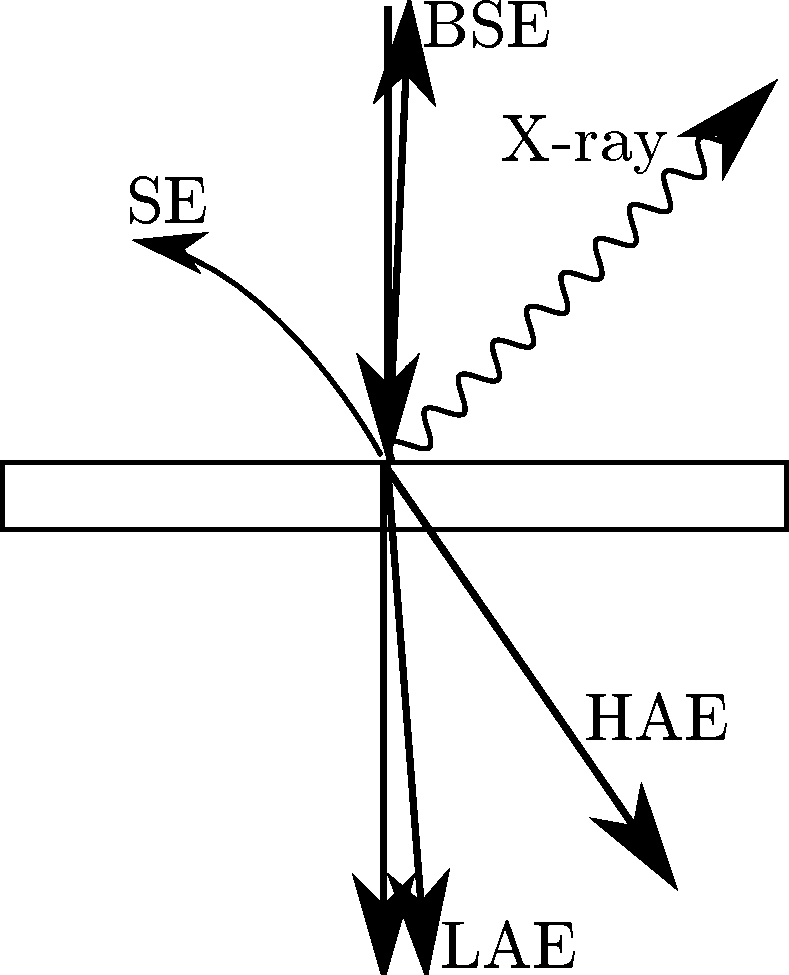
\includegraphics[width=0.5\textwidth]{exp_em_electron_interaction}
 \caption[Electron interactions with materials]{\label{fig:exp_em_electron_interaction}Schematic of an electron beam interacting with a sample showing backscattered electrons (BSE), secondary electrons (SE), generated X-rays, low angle scattered electrons (LAE), high angle scattered electrons (HAE), and the main electron beam passing through the sample.}
\end{figure}

This work relied upon two measurement techniques which utilized electrons as their primary probe, scanning electron microscopy (SEM) and (scanning)transmission electron microscopy (STEM/TEM).
SEM is an invaluable non-destructive technique for examining surfaces at high resolution to extract information about both the structural and chemical properties.
STEM/TEM is a tool which uses similar interactions to examine the cross sectional structural and chemical properties of mechanically thinned slices of materials with sufficient resolution to examine individual columns of atoms in crystals.
\subsection{SEM} Scanning electron microscopy is a high resolution non-destructive and non-contact technique used to examine the surface of a sample.
SEM can reveal the topography and chemical composition of a surface down to 10's of nanometers, and the chemical composition on the micrometer scale.
These measurements are achieved through the interaction of a beam of nearly-monochromatic electrons generated from a heated filament or cold cathode and accelerated to kilovolt energies in an high vacuum chamber and focused onto a sample.
Magnification is achieved in SEM by careful scanning of the focused beam over a small area.

\subsubsection{Secondary Electron Imaging} The most common electron-material interaction utilized in SEM is generation of images through the production and capture of secondary electrons.
Secondary electrons are continuum (valence and conduction band) electrons excited from the sample through inelastic scattering excitations as an electron beam penetrates into a sample.
These electrons typically have energies of less than 50~eV\cite{goldstein2003scanning}.
Secondary electrons, while generated along the path of incoming electrons, can only typically escape from depths of less than 7.5~nm, making secondary electrons surface sensitive\cite{goldstein2003scanning}.
Secondary electrons are collected by biasing an electron detector to electrostatically attract these low energy electrons while not appreciably affecting the incoming beam.
Electron detectors are typically a phosphor screen combined with a photomultiplier tube to provide high gain.
Images are formed by scanning the beam across the surface of the sample and counting the secondary electron yield for each dwell point within the scan.
The resulting grid of counts is transformed into a bitmapped grayscale image.

As secondary electrons are low energy, their escape depth from a surface is very shallow, as such their yield is very sensitive to the local topography of the sample.
Thus to the first approximation, the contrast in a grayscale image formed from secondary electrons is a representation of the topography present on the surface of the sample.
Regions with vertical extent will increase the yield of secondary electrons, due to more of the sample being within nanometers of the surface.
An extreme case of this is vertical edges, which will have a high yield of secondary electrons, due to having the top and side surfaces both yielding secondary electrons.

\subsubsection{Backscattered Electron Imaging} High energy incoming electrons can also interact with samples via elastic scattering.
Electrons which are scattered at close to 90\degree{} are backscattered close to the incoming beam.
By placing an unbiased detector near the incoming electron beam the detector can capture backscattered electrons.
The electron elastic scattering process is proportional to atomic mass (\(\sim\)\(\sqrt{Z}\))) of the sample.
The yield of backscattered electrons provides mass (usually called compositional) contrast of the sample under the electron beam.
Penetration depth of the electron beam for backscattered electrons is deeper than secondary electrons, generally penetrating 1--2~\micro{}m into the sample, as well as laterally broadening.
Such broadening reduces the resolution of backscattered imaging compared to secondary electron imaging.

\subsubsection{Practical SEM} The practical application of SEM for imaging of samples requires the optimization of several parameters.
While SEM is a non-destructive measurement technique, intentional sample preparation can vastly improve the imaging resolution and reduce noise.
A key requirement for SEM samples is that the sample is sufficiently conductive to conduct away the electrons delivered by the scanning beam.
For high conductivity samples, sample preparation can be as simple as bonding to a sample holder using conductive tape or paste (such as carbon tape or silver paste).
Samples with poorer bulk conductivity may require conductive paste applied to contact the top surface to the sample holder.
Highly insulating samples are normally coated with a thin layer of high density metal (Pt, Au) or amorphous carbon in order to provide a conduction path to the conductive paste connecting the top surface to the sample holder.

Optimization of imaging for a given sample is achieved through the tuning of several imaging parameters, working distance, accelerating voltage, beam current and dwell time\cite{goldstein2003scanning}.
For typical secondary electron imaging, the goal is to interact with the thin top surface layer with the smallest lateral beam possible.
Minimization of accelerating voltage, beam current and working distance will maximize the resolution and reduce the surface interaction.
Reduction of these working parameters has the side effect of reducing the signal to noise ratio (SNR) of imaging.
Increasing dwell time can improve SNR, but for poorly conductive samples charge buildup will cause deflection of the incoming beam.
Stacked averaging of quick scans yields improved SNR on the tradeoff of time.

Interpretation of the secondary electron images in one key case is ambiguous; topographic features with vertical extent can appear to be both a depression and a bump simultaneously, due to the assumption of the human visual system that lighting always comes from above\cite{goldstein2003scanning}.
Care must be taken for features of this type to avoid misinterpretation.
Modification of some imaging parameters can break the ambiguity and reveal the topography, including tilting the sample, rotating it about its surface normal using the SEM's focus and depth of field parameters to slice through the topography.

Imaging of samples using backscattered electrons to achieve chemical composition requires optimization of the elastic scattering process from the sample.
The primary parameter that improves backscattered electron yield is increases of the electron accelerating voltage.
Increasing the accelerating voltage has the downside of increasing the area of electron interaction, which reduces the effective spatial resolution\cite{goldstein2003scanning}.
The elastic scattering process is less efficient per incident electron than secondary electron generation, as such beam dwell times must be increased to improve SNR\@.
To obtain a accurate measure of chemical composition, samples for backscatter analysis should be as flat as possible, as topography can modify the yield of backscattered electrons, processing such as polishing is essential for the highest accuracy chemical composition.
If the measurement is intended to be non-destructive, careful correlation between backscattered and secondary electron images must be used to ignore topographic effects.
\subsection{TEM} While scanning electron microscopy relies on the information generated from the surface and sub-surface of arbitrarily thick samples, transmission electron microscopy (TEM) relies on the information generated from electrons which transmit through a sample.
Through control of the electron beam information about the thickness, crystalinity, and defects of a sample can be collected.

Imaging of samples via TEM is produced via one of several interaction mechanisms of a beam electrons with a thin sample, as noted in the transmitted electron beams in \cref{fig:exp_em_electron_interaction}.
Electron beams are generally on the order 10's to 100's of kilovolts and are controlled via magnetic lenses\cite{Egerton2005}.
Images can be formed by collecting the scattered beam (dark-field) or the transmitted beam (bright-field) focused onto a scintillating screen or electronic CCD array.
Magnification in TEM is achieved by controlling the width of the beam that passes through the sample and then expanding it again onto the detector.
Magnification is generally limited by aberrations present in the magnetic lenses of the system.

Without any specific alignment of the sample, TEM image intensity provides contrast of the thickness-density product of the sample\cite{Egerton2005}.
Electrons are absorbed or scattered away more strongly where there are more atoms present in the path of the electron beam, either through more electrons per unit thickness, or more thickness in total.
Thus, some contrast formed in the image is an indication of the composition.

While thickness-density contrast can provide some information, it is generally useful for amorphous or biological samples.
Crystalline materials offer several other contrast mechanisms.
The de~Broglie wavelength of electrons accelerated in a TEM is much smaller than the spacing between atoms in typical materials, so those electrons can undergo diffraction when they interact with a crystalline sample.
Polycrystalline samples will provide distinct intensity contrast due to their large changes in orientation relative to the incoming electron beam, diffracting varying amounts of electrons\cite{Egerton2005}.

When samples are more crystalline, polycrystalline diffraction contrast generally no longer plays a large role.
In order to improve the contrast effects of electrons passing through crystalline samples, the sample must be aligned along a ``zone-axis,'' that is, along some crystal direction in order to transport electrons mostly unperturbed down atomic columns.
TEM samples are tilted to align the sample so the beam travels along a crystal direction.
When crystalline samples are aligned in such a way, defects that break the periodicity of the crystal result in scattering of the electrons and create what is called phase contrast.
Phase contrast will highlight regions where the atomic columns have defects which scatter electrons\cite{Egerton2005}.

When a sample has crystal defects which present the same zone axis, such as twins, they do not show up in diffraction contrast or traditional phase contrast.
In these cases, single zone axis imaging cannot provide a contrast mechanism which differentiates the two phases.
Two-zone axis contrast tilts the sample in a second direction perpendicular to the first and brings the sample into a dual-diffraction condition.
Since such crystal phases differ in the direction perpendicular to the zone axis, the dual-zone diffraction uses this difference to provide contrast.

Beyond imaging, the electron beam can be adjusted such that after the electrons pass through the sample, the electrons that diffract with the crystal planes can be focused into spots resulting in a diffraction pattern.
This diffraction pattern is akin to an X-ray pattern, it can be used to determine the crystal structure and orientation of the sample under the beam.
The size of the electron beam can also be limited, a method known as selected area diffraction (SAD), allowing examination of sections of the sample.
\subsubsection{Practical TEM} While TEM is a excellent technique for investigating the microstructure of epitaxial thin films, it imposes strict limitations on sample preparation.
Samples must have lateral dimensions of several millimetres while being thinned to electron transparency.
The precise thickness depends upon the density of the material and the TEM conditions.
Samples must be generally thinner than 100~nm for enough electron transmission to provide enough electron scattering to provide contrast while also having those scattered electrons pass through to a detector.

Samples generally start out as wafers or sections of wafers with thicknesses of 500~\micro{}m and lateral dimensions of up to several inches.
Before thinning of a TEM sample can be undertaken, a section of a (possibly) large bulk sample must be selected.
The section selected must be of a size compatible with the thinning process.
Preparation of such sections depends upon the properties of the substrate.
For substrates with good cleaving properties, a thin bar can be cleaved, for substrates which are much harder, bars must be sectioned using sawing methods such as diamond or wire saws.

Once sections have been extracted from a larger sample, they must be progressively thinned.
This is done through a number of steps, starting with mechanical polishing.
In traditional sample preparation a sample is preferentially polished in a wedge shape, providing a gradient of thickness, where at some point the ideal thickness is present.
In modern preparation techniques the sample is ``dimpled,'' creating a sample with circular gradient of thickness and then ion milled until break through.
Samples prepared by most methods are gentle argon ion milled to remove polishing damage.

When preparation of a specific region of a sample is required, traditional preparation techniques do not provide enough spatial specificity to select features at the micro or nano level.
For sample preparation of this type, preparation is performed using a Focused Ion Beam (FIB) milling system.
A hybrid gallium beam/SEM system is used to selectively mill the region of interest and perform localized sputtering of a sample, slicing out a section.
After isolating the section, it is welded to a nanomanipulator probe and transferred onto a TEM grid.
The sample is then thinned to electron transparency with the FIB beam, before finally being cleaned by argon gentle ion milling.

Preparation techniques must be extensively experimented with when preparing new or unknown samples.
Some epitaxial layers will have greatly differing mechanical properties and react differently to mechanical polishing and ion sputtering.
Care must be taken to not preferentially remove the material of interest.
Haphazard preparation can result in the introduction of artifacts which may cause misinterpretation during imaging.

Beyond sample preparation, imaging in a TEM can be modified by tuning several parameters.
The accelerating voltage of the TEM affects the wavelength of the electron beam, improving resolution with increasing accelerating voltage\cite{Kohl2008}, however resolution is ultimately limited by lens aberrations.
Lens aberrations can only be improved by the introduction of correctors such as electron monochrometers (which reduce electron current by throwing away those outside a set energy range) and aberration correctors which significantly increase cost.
Beam current control is important to provide good signal to noise, but excess current can cause heating and damage in ultra-thin samples.

\subsection{STEM}
While TEM image formation passes a large beam of electrons through a region of a sample, scanning transmission electron microscopy (STEM) forms an image more akin to SEM\@.
The electron beam is rastered across the thin sample and an image is formed by measuring electron beam current on one of several detectors.
Because the electron beam is a focused point rather than a beam, with the detector immediately after the sample, the maximum resolution achievable in such a system is substantially higher than traditional TEM, reaching levels of \(<\)~1\AA{}.
While STEM's rastering system is beneficial for improving traditional bright-field and dark-field imaging, its major benefit is the addition of the High Angle Annular Dark Field (HAADF) detector for imaging.
The HAADF detector is located after the sample at a larger angular deviation in comparison to the small angle scattering used in TEM, this high angle scattering arises due to atomic Z number scattering of the electrons.
The resulting image formed by collecting data with a HAADF detector is a Z-contrast image, with the brighter spots corresponding to higher Z-number atomic columns within a sample.
The Z-contrast provided by STEM allows identification of atoms within a crystal structure based upon the relative intensities.

In addition to the Z-contrast imaging available within STEM, the electron beam which passes through the sample has energy losses which are characteristic of the atoms which the beam passed.
If a spectrometer is placed below the sample, the energy loss can be measured and a Z-contrast image can be correlated with simultaneous spectroscopic energy loss information, providing chemical pseudo-contrast after post processing.
Such a process is known Electron Energy Loss Spectroscopy (EELS).

\subsubsection{Practical STEM} 
The preparation conditions for STEM is even more onerous than those for traditional TEM\@.
The electron yield for HAADF imaging and EELS quickly diminishes with increasing thickness of the sample.
Samples must be thinned by progressive low energy ion milling to ensure no remaining damage or amorphous layers are present.
Such thin layers must also be stored in vacuum and analyzed quickly as such thin samples can quickly react with water and oxygen in air and chemically react or adsorb contaminants.

STEM imaging is most useful when paired with traditional TEM imaging, as phase and diffraction contrast can highlight regions of interest and Z-contrast imaging can examine the fine details at boundaries between such regions.
Additionally, combining STEM with 2DXRD and careful sample preparation which maintains orientation relationships can provide absolute crystal orientation information, including polarity of polar crystals.

\section{Growth Techniques}
The work presented in this thesis are prepared primarily by two different growth methods, pulsed laser deposition (PLD) and molecular beam epitaxy (MBE).
While these methods are distinct in their properties and the regimes under which they operate, the same material systems were not prepared by both systems, so direct comparisons cannot be made.
Nevertheless, the differences between these growth processes will be examined in some detail to provide sufficient motivation for their choice for the given experiments.
\subsection{PLD} Pulsed laser deposition (PLD) is a versatile method of growing epitaxial thin films and nanostructures.
PLD has the ability to operate in a non-equilibrium growth regime, that is, at a point where the atoms are excited to energies much above the temperature of the growth substrate.
Such a regime is achieved by the use of a pulsed, high photon energy and high energy density laser to produce the atomic species used for growth.
The properties of the PLD growth system allow a wide range of temperatures, pressures and material types to be used during attempts at epitaxial growths.
\begin{figure}
 \centering 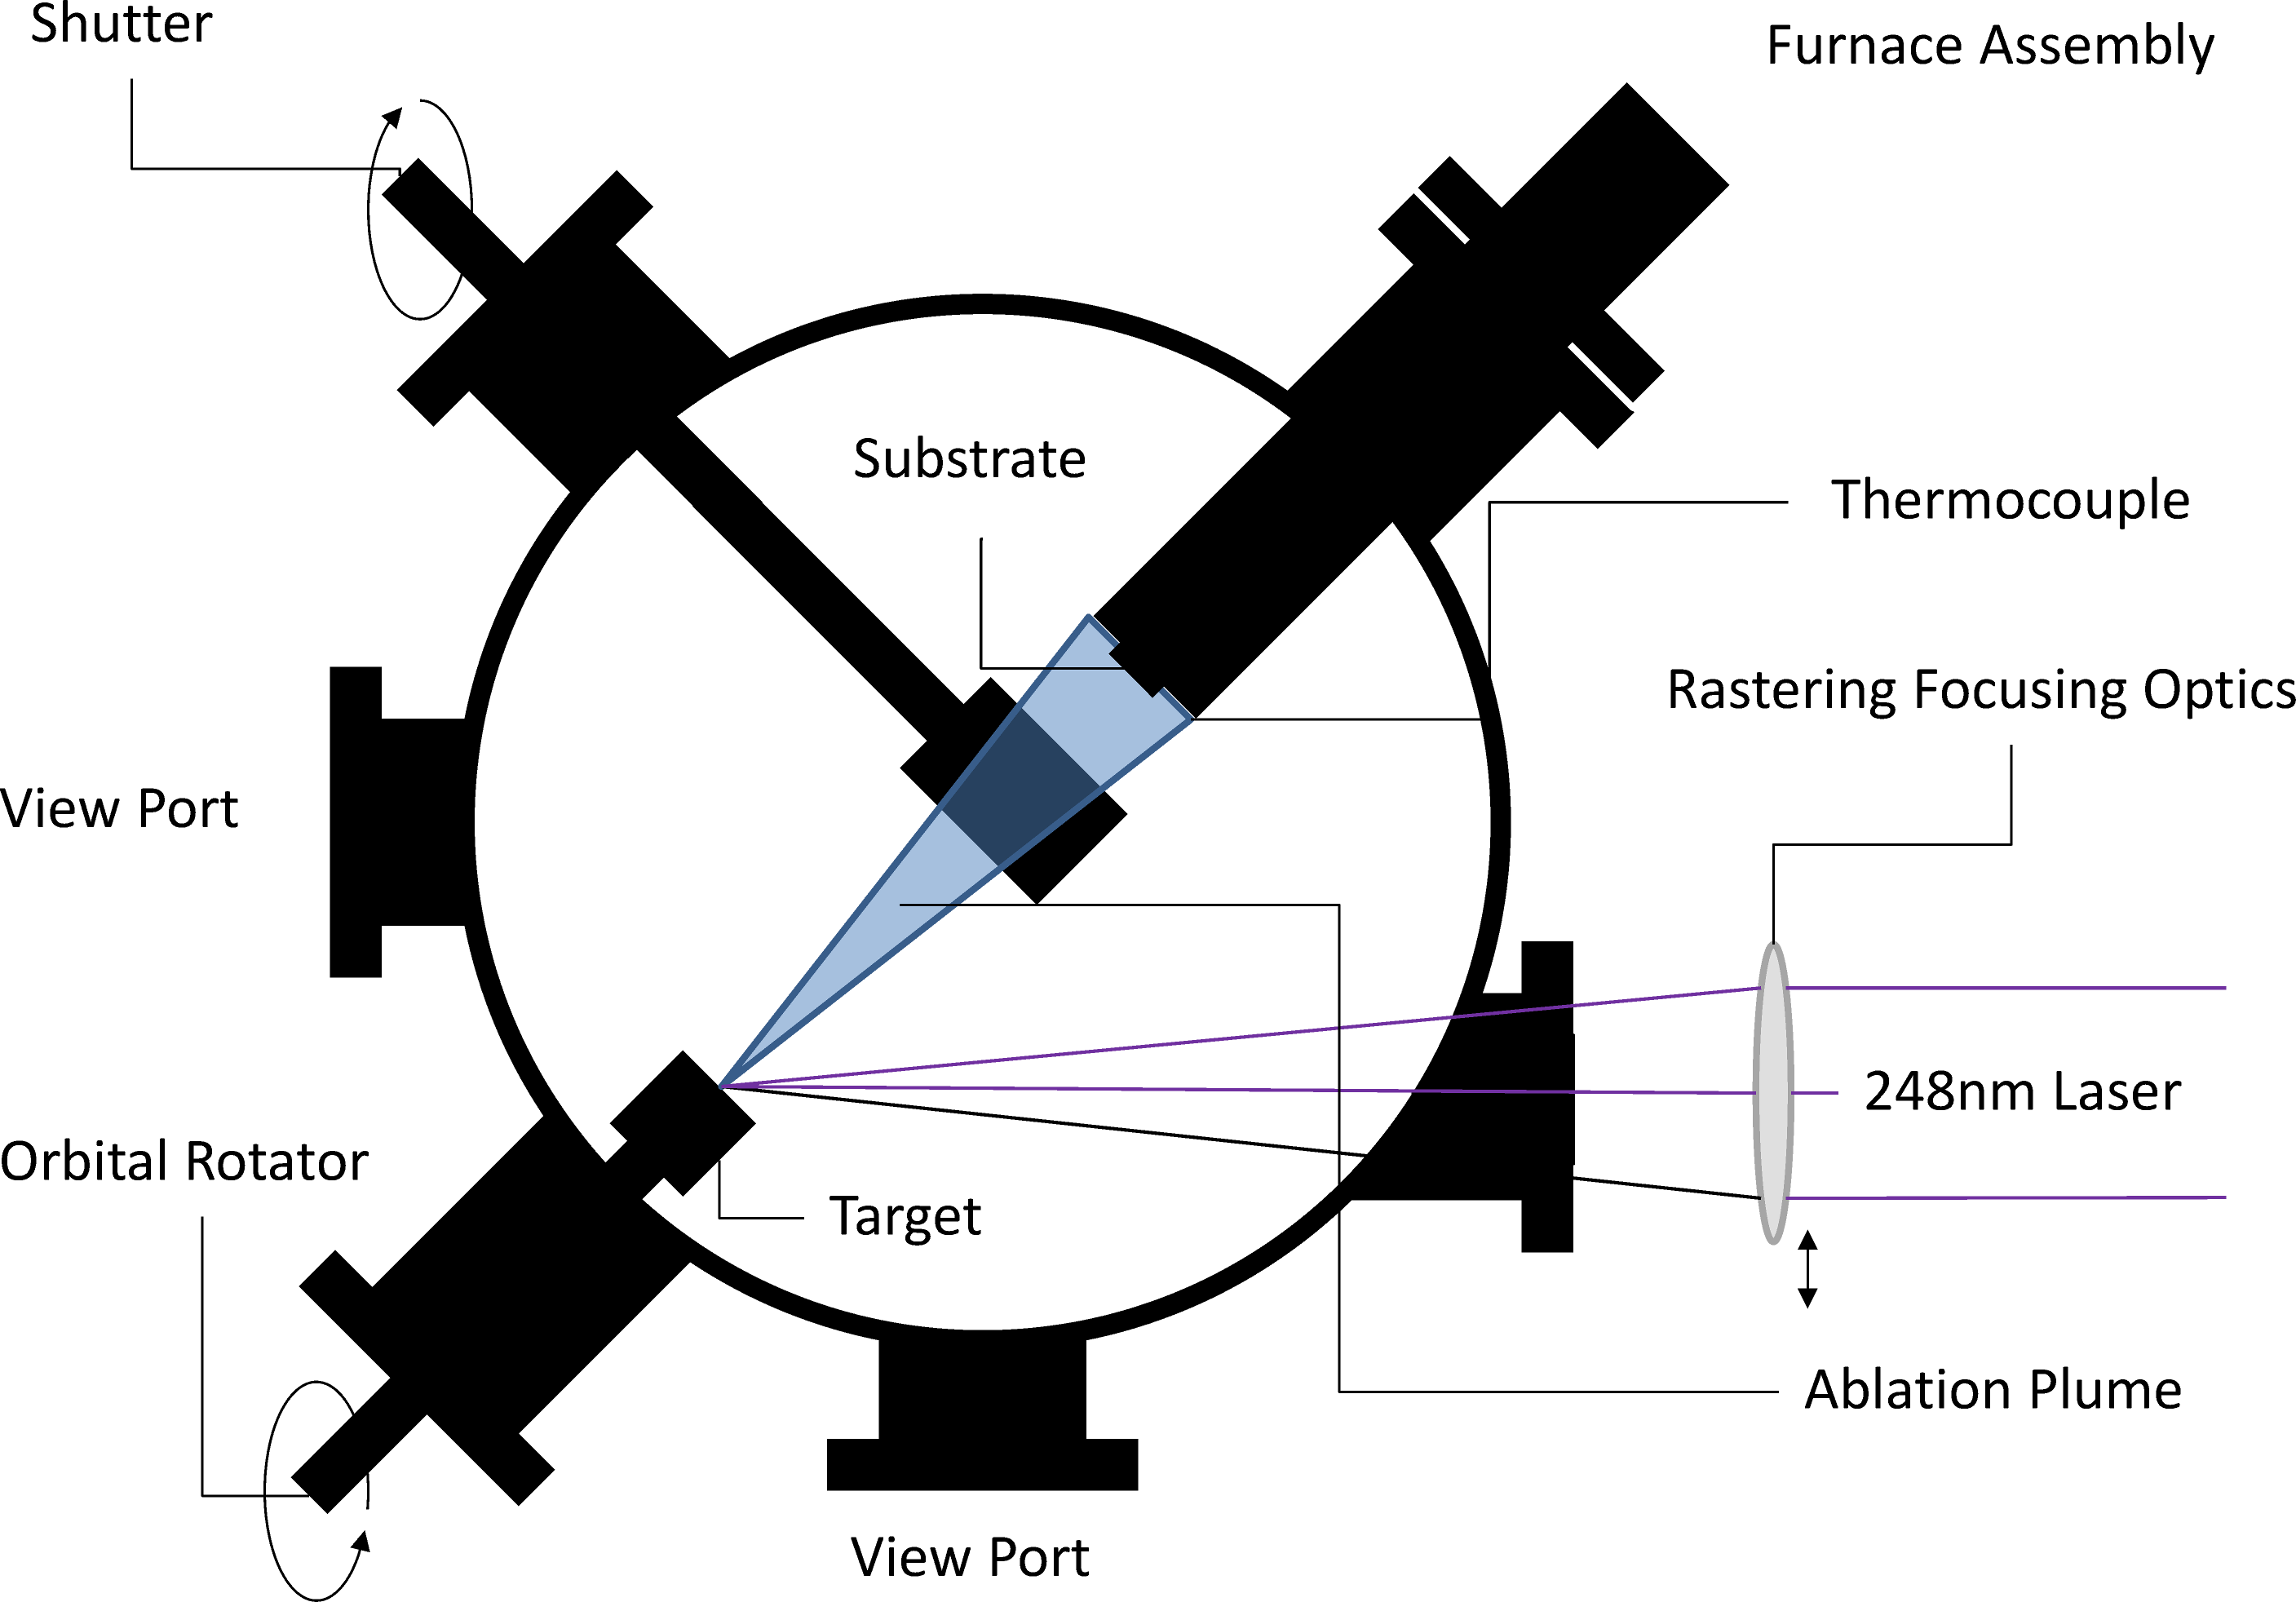
\includegraphics[width=0.9\textwidth]{exp_PLD_chamber}
 \caption[PLD chamber schematic]{\label{fig:exp_pld_chamber}PLD Chamber Schematic (used with permission after~\cite{stephen-thesis}).}
\end{figure}

The PLD process uses a process known as laser ablation to produce the atomic species used for epitaxial growth.
The laser ablation process relies on several key parameters of the laser and to a lesser extent a few material parameters.
The lasers used in PLD have pulse widths of \(<\)~50~ns, with UV photon energies and total energies of 50---500~mJ/pulse.
Typical PLD lasers are excimer lasers with 248~nm UV photons and pulse widths of \(\sim\)25~ns.
Growth rates for PLD are limited by the pulse rate of the laser, and secondarily by the ability of the target to withstand the sustained energy deposition without melting.

The laser ablation process is achieved by application of laser pulses focused onto a target material, to achieve energy densities \(>\)~1~J/cm\textsuperscript{2}.
The photon energy is absorbed within a thin surface layer 1/\textalpha{}, producing plasmons, excited electrons and excitons\cite{Willmott2000}.
These high energy electrons thermalize and release their energy into the lattice within a few picoseconds.
After this thermalization step, the ablation depth is modified by thermal diffusion, highly conductive metals can quickly spread heat up to a micron deep.
The deposited energy then results in a pulse of evaporation from the target, called the plume.
For highly thermally conductive samples, the surface layer can begin to ablate before the laser pulse is fully absorbed, in these cases further absorption in bulk is screened by the atomic plume\cite{Willmott2000}.

Regardless of the target material, a plume is generated at the laser spot which, due to the laser pulse and heating timescales, is stochiometric with regards to the composition of the target.
The atomic plume is also highly ionized, with energies of 1--100~eV and with typical energies of 5--50~eV\@. The atomic plume is now a vapour but highly compressed next to the target surface.
It explodes perpendicular to the surface, expanding across the deposition chamber, to be collected by a waiting substrate.
The plume expands from the target with a \(\cos^{10}(\theta)\) -- \(\cos^{20}(\theta)\)
dependence, meaning it is highly peaked centrally about the laser spot.
Once the atomic plume arrives at the substrate, its energy is delivered to the growing film.
The high energy atoms, in addition to having high rates of diffusion, also promote the movement of atoms already present by providing activation energy for their diffusion processes\cite{Willmott2000}.
This is a key reason the PLD process can be used at substrate temperatures lower than other methods, as the atomic plume delivers energy directly to the growing film.

Due to the generation of atomic species using light, the environment surrounding the target and growth substrate need not be ultra-high-vacuum or even high vacuum for the excited plume to successfully traverse the gap between target and substrate.
Gas pressures on the order of mTorr can be used to modify the energetics of the atomic plume, reducing the total energy or modifying the distribution\cite{Willmott2000}.
The addition of reactive gasses into the chamber, in addition to participating in plume modification, can also participate chemically in the growth process, allowing the growth of oxides and other gas-incorporating materials.
Doping of materials grown with PLD is achievable by incorporating the dopant elements into the existing targets, or by periodically co-ablating pure targets using a target exchange system.

The main limitation of PLD are due to the highly peaked nature of the laser plume, that is, the spatial extent of the atomic plume is limited.
The plume must be rastered across large substrate into order to grow a uniform layer.
A secondary limitation is the production of macroscopic droplets which can impact the epitaxial growth process.
The droplets are produced by several processes, some of which can be mitigated.
Targets must be of very high density in order to ensure superheated gasses from voids do not eject pieces of the target.
For highly thermally conductive samples (typically metals), the laser pulse can cause sub-surface boiling, resulting in ejection of liquid material from the target.
For systems which experience this issue, energy per pulse must be reduced to the minimum which can achieve ablation.
A similar process which produces macroscopic droplets is recoil ejection, again for fast conducting materials.
As the vaporization shockwave in a target moves into already melted material, the forces can cause a compression and rebound of the liquid material into a macroscopic droplet.

\subsection{MBE} Molecular beam epitaxy (MBE) is considered the gold standard for the growth of carefully controlled epitaxial thin films and nanostructures, being used for both research and commercial purposes.
Its implementation as a growth process allows for a wide range of growth rates from angstroms per second to microns per minute, while controlling the precise ratio of incoming atomic species, and allowing for abrupt changes in composition.

MBE growth systems consist of a large ultra high vacuum (UHV, \(<\) 1e-8 Torr) chamber, along with associated load lock system and exchange hardware, which can accept growth substrates of sizes up to several inches.
This low pressure environment is essential to the MBE process to ensure a mean free path of larger than the chamber for the atomic beams used during growth.
These atomic beams are generated in the chamber by one of two processes, effusion cells, or gas sources.
In an effusion cell, a high temperature ceramic containing a solid ultra-pure source of material, is heated to cause evaporation, which then travels in the molecular beam regime across the chamber to a substrate.
Effusion cell rates are controlled by the temperature of the cell.
In gas sources, an organometallic gas containing the atomic species of interest is passed into the chamber via a ``cracker,'' a heated filament used to burn the organic components of the gas, leaving the atomic species which travel across the chamber and are collected on a substrate.
Gas source rates are controlled by mass flow controllers adjusting the rate of gas passing into the system.
Growth rates of angstroms per minute to micrometers per hour are possible via high flow crackers and industrial growths.

MBE systems are used to grow materials in a wide variety of systems, typically concentrated in the III-V, and can also include a wide variety of electrical dopants during growth.
Strict control of the atomic sources allows growth of repeating multilayer stacks, graded materials and quantum structures.
In addition to the careful control of the atomic species, MBE's low pressure system allows in-situ monitoring and characterization of the growth surface using electron-based techniques such as reflection high energy electron diffraction (RHEED).

The main limitation of MBE is the ability to only produce a single sample at a time, making it unsuitable for high volume commercial production.
Another limitation is the heating and temperature control of the substrate.
Since samples must be added via load lock, contact heating and temperature measurement is impractical, leaving only indirect radiative heating and pyrometry temperature measurement.
